 \documentclass [12pt]{article} 

\usepackage {amsmath}
\usepackage {amsthm}
\usepackage {amssymb}
\usepackage {graphicx} 
\usepackage {float}
\usepackage {multirow}
\usepackage {xcolor}
\usepackage [ruled,vlined,commentsnumbered,titlenotnumbered]{algorithm2e} \usepackage {array} 
\usepackage {booktabs} 
\usepackage {url} 
\usepackage {parskip} 
\usepackage [margin=1in]{geometry} 
\usepackage [T1]{fontenc} 
\usepackage {cmbright} 
\usepackage [many]{tcolorbox} 
\usepackage [colorlinks = true,
            linkcolor = blue,
            urlcolor  = blue,
            citecolor = blue,
            anchorcolor = blue]{hyperref} 
\usepackage {enumitem} 
\usepackage {xparse} 
\usepackage {verbatim}
\usepackage{algpseudocode}
\usepackage{listings}
\usepackage{xcolor}
\lstset { %
    language=C++,
    backgroundcolor=\color{black!5}, % set backgroundcolor
    basicstyle=\footnotesize,% basic font setting
}
\newtheorem{theorem}{Theorem}
\newtheorem{remark}{Remark}
\newtheorem{lemma}[theorem]{Lemma}
\newtheorem{corollary}[theorem]{Corollary}
\theoremstyle{definition}
\newtheorem{definition}{Definition}[section]
\newtheorem{claim}{Claim}
\newtheorem{proposition}{Proposition}






\DeclareTColorBox {Solution}{}{breakable, title={Solution}} \DeclareTColorBox {Solution*}{}{breakable, title={Solution (provided)}} \DeclareTColorBox {Instruction}{}{boxrule=0pt, boxsep=0pt, left=0.5em, right=0.5em, top=0.5em, bottom=0.5em, arc=0pt, toprule=1pt, bottomrule=1pt} \DeclareDocumentCommand {\Expecting }{+m}{\textbf {[We are expecting:} #1\textbf {]}} \DeclareDocumentCommand {\Points }{m}{\textbf {(#1 pt.)}} 

\begin {document} 

\vspace {1em} 
\begin {Instruction} 
Adapted From Virginia Williams'lecture notes.
\end {Instruction}  

{\LARGE \textbf {COMP 285 (NC A\&T, Spr `22)}\hfill \textbf {Lecture 32} } 

\begin{centering}
\section*{MSTs II, Max Flow}
\end{centering}

\section{Kruskal's Algorithm} 

At a high level, the set A maintained by Kruskal's algorithm is a set of disjoint trees. During update step $i$, if the ith smallest edge connects different trees, merge the two trees connected by this edge. The algorithm progresses until eventually only one tree remains at which point the set A represents an MST of the graph.

Kruskal's algorithm utilizes the union-find (aka disjoint set) data structure in order to handle the merging of the disjoint trees maintained by the algorithm. The union-find data structure supports disjoint sets with the following operations:

\begin{itemize}
\item \textbf{makeset}$(u)$: creates a new set containing $u$ provided that $u$ is not in any other set
\item \textbf{find}$(u)$: returns the name of the set containing $u$
\item \textbf{union}$(u, v )$: merge the set containing $u$ and the set containing $v$ into one set
\end{itemize}

The algorithm itself can be structured as follows:

\begin{algorithm}
\caption{Kruskal($G$)}
\label{alg:kruskal_algorithm}
\begin{algorithmic}
\State $A \gets \emptyset$
\State $E' \gets$ sort edges by weight in non-decreasing order
\State \For{ $v \in V$} {
    \State makeset(v)
}
\State \For{ $(u,v) \in E'$} {
    \If{find($u) \neq $ find(v)} {
        \State $A \gets A \cup \{(u,v)\}$
        \State union(u,v)
    }
}
\State \Return $A$
\end{algorithmic}
\end{algorithm}

\textbf{Correctness} The correctness follows from Theorem \ref{thm:lemma}.


\textbf{Running time} 

The runtime of Kruskal's algorithm depends on two factors: the time to sort the edges by weight and the runtime of the union-find data structure operations. While $\Omega(m \log n)$ time is required for sorting the edges if we use comparison-based sorting, in many cases, we may be able to sort the edges in linear time. (Recall, that RadixSort can be used to sort the edges in $O(m)$ time if the weights are given by integers bounded by a polynomial in $m$.) In this case, the runtime is bounded by the runtime of the union-find operations and is given by $O(nT(\text{makeset}) + mT(\text{find}) +nT(\text{union}))$. The best known data structure supporting the union-find operations runs in amortized time $O(\alpha(n))$ where $\alpha(n)$ is the inverse Ackermann function. Interestingly, the value of the inverse Ackermann is tiny for all practical purposes: 
$$
\alpha(n) \leq 4, \forall n < \text{\# atoms in the universe}
$$

and thus for all practical purposes, the union-find operations run in constant time. Thus, in many settings, the runtime of Kruskal's algorithm is nearly linear in the number of edges. 

The actual definition of $\alpha(n)$ is $\alpha(n) = \min\{k \mid A(k) \geq n\}$, where $A(k)$ is the Ackermann function evaluated at $k$. $A(k)$ itself is defined using the more general Ackermann function as $A(k) = A_k(2)$. $A_k(x)$ is defined recursively: 

\begin{align*}
A_m(x) = 
    \begin{cases}
        x + 1 & m = 0 \\
        A_{m-1}(1) & m > 0, x = 0  \\
        A_{m-1}(A_m(x - 1)) & \text{ else }
    \end{cases}
\end{align*}

For example
\begin{itemize}
    \item $A_0(x) = 1 + x$, so $A_0(2) = 3$
    \item TO compute $A_1(x)$, we see:
    $$
    A_1(x) = A_0(A_1(x-1)) = A_0(A_0(A_1(x-2))) = \cdots = A_0(A_0(\cdots (A_0(A_1(0))))) = A_0(A_0(\cdots(A_0(2))))
    $$
    that is, we have ``iterated'' $A_0 x$ times. If we work it out, we get:
    $$
    A_1(x) = 2x
    $$
    Thus, $A_1(2) = 4$
    \item $A_2(x) = 2^x x$ ($A_1$ iterated $x$ times), so $A_2(2) = 8$ 
    \item $A_3(x) \geq 2^{2^{2^{2\cdots}}}$, a "tower" of $x$ 2s ($A_2$ iterated $x$ times); it turns out that $A_3(2) \geq 2^11$
    \item $A_4(x)$ is larger than the total number of atoms in the known universe, and also greater that the number of nanoseconds since the Big Bang. (Thus, $\alpha(n) \leq 4$ for all practice purposes)
\end{itemize}

\textbf{Example} In this example (Figure \ref{fig:kruskal0}) we will run through the steps of Kruskal's algorithm in order to find an MST for the following graph:


\begin{figure}[h!]
\centering
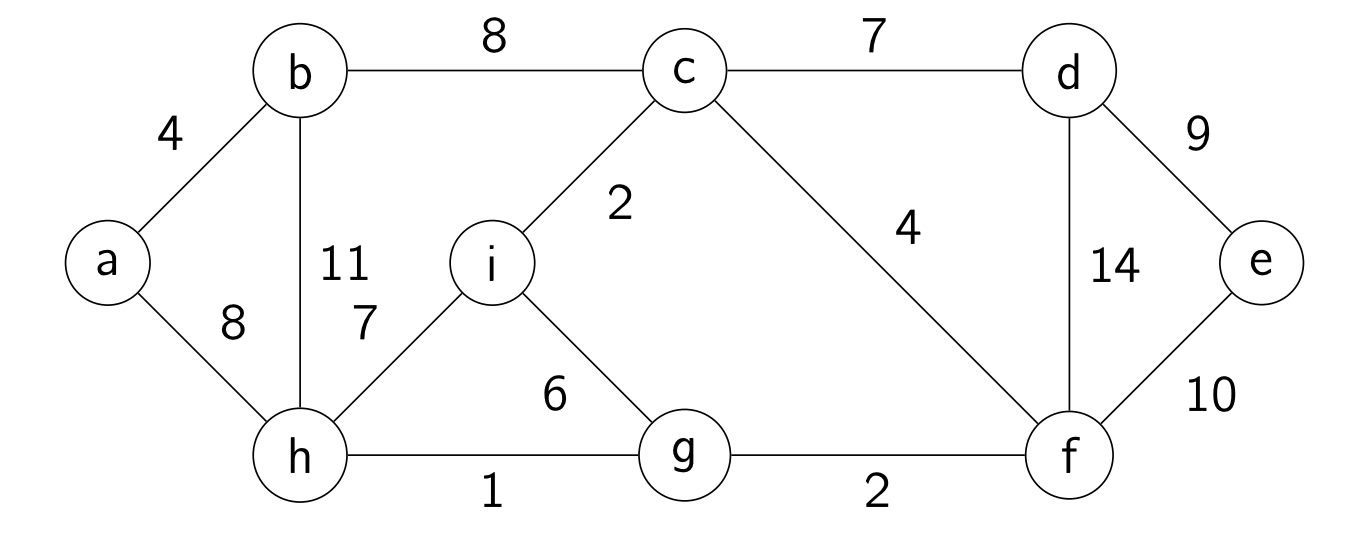
\includegraphics[scale=0.8]{kruskal0.png}
\caption{}
\label{fig:kruskal0}
\end{figure}
 
We begin by creating a new set for each node in the graph. We then begin iterating over the edges in non-decreasing order. The first edge we examine is $(g, h)$. This edge connects nodes $g$ and $h$ which are currently not part of the same set. We thus include this edge in $A$ and union the sets containing $g$ and $h$ as shown in Figure \ref{fig:kruskal1}.

\begin{figure}[h!]
\centering
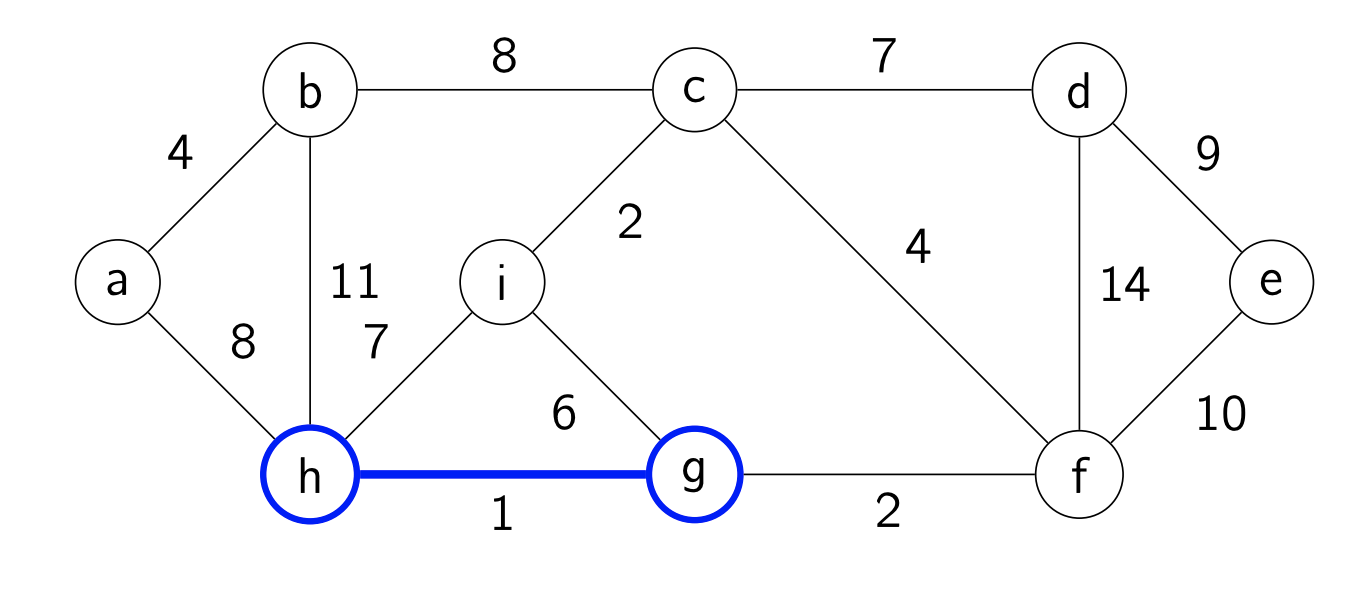
\includegraphics[scale=0.8]{kruskal1.png}
\caption{}
\label{fig:kruskal1}
\end{figure}

The next edge in the sorted order is a tie between edges $(c, i)$ and $(f , g)$. Picking either one will yield a correct result, so let's say the algorithm picks $(c, i)$. Since $c$ and $i$ are not part of the same set we include this edge in $A$ and union the sets containing $c$ and $i$ as shown in Figure \ref{fig:kruskal2}.

\begin{figure}[h!]
\centering
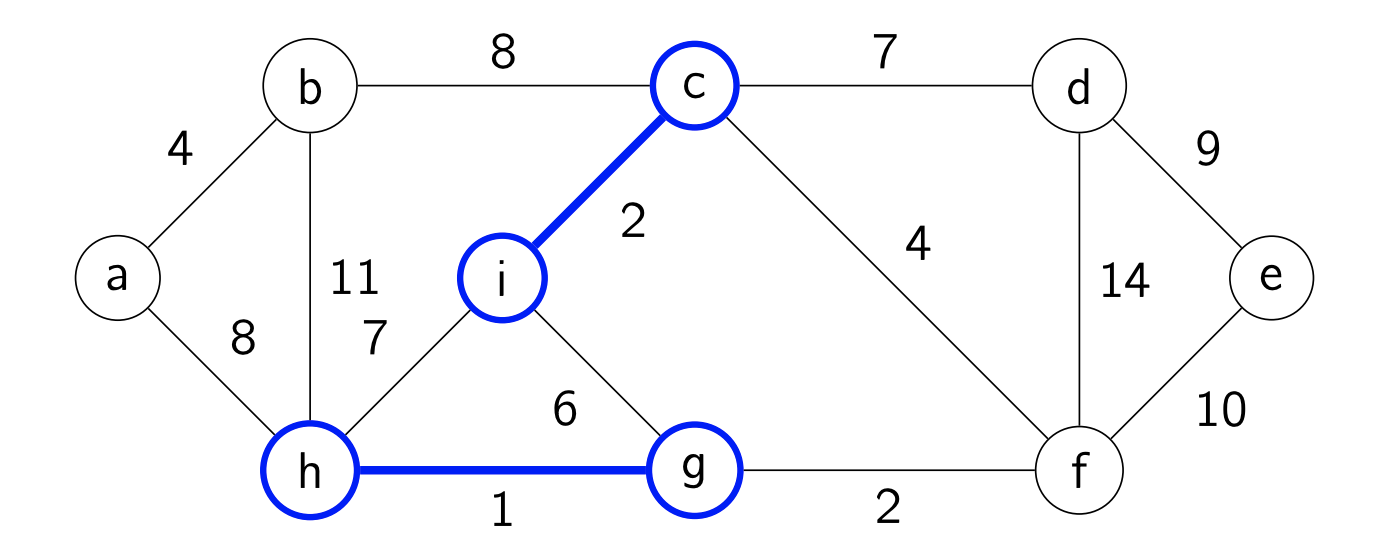
\includegraphics[scale=0.8]{kruskal2.png}
\caption{}
\label{fig:kruskal2}
\end{figure}



The next edge in the sorted order is $(f , g)$. We union the sets containing $f$ and $g$ and add edge $(f , g)$ to $ A$ as shown in Figure \ref{fig:kruskal3}.


\begin{figure}[h!]
\centering
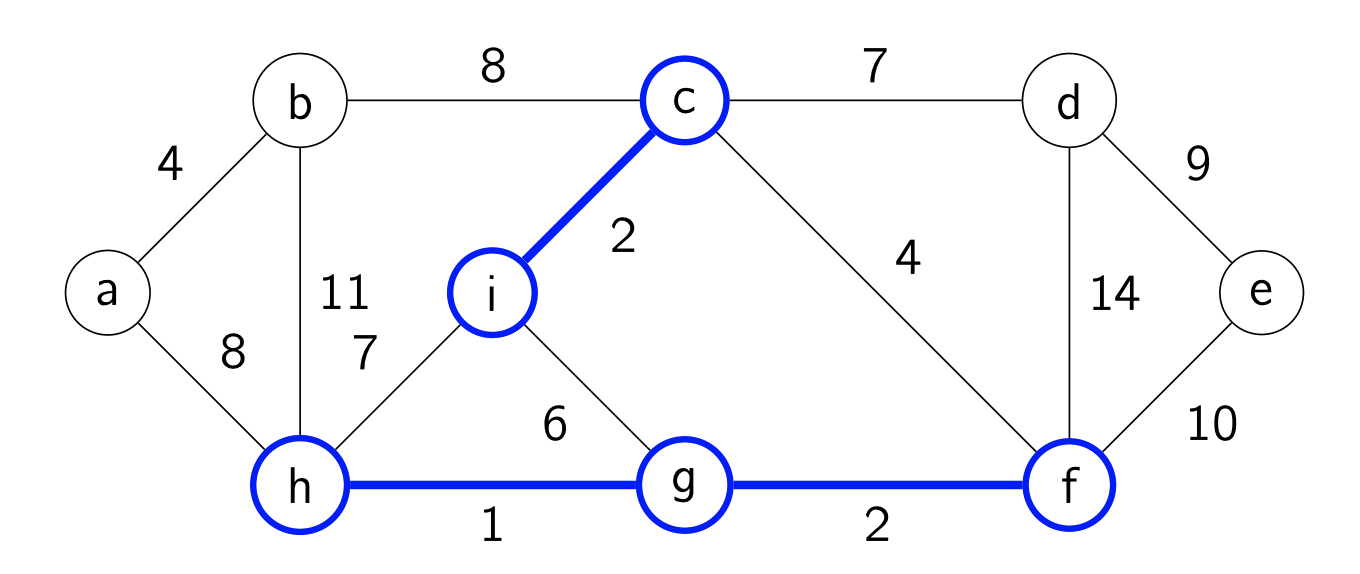
\includegraphics[scale=0.8]{kruskal3.png}
\caption{}
\label{fig:kruskal3}
\end{figure}

The next edge in the sorted order is a tie between edges $(a, b)$ and $(c, f )$. Let's say the
algorithm picks $(a, b)$. We union the sets containing $a$ and $b$ and add edge $(a, b)$ to $A$ as shown in Figure \ref{fig:kruskal4}.

\begin{figure}[h!]
\centering
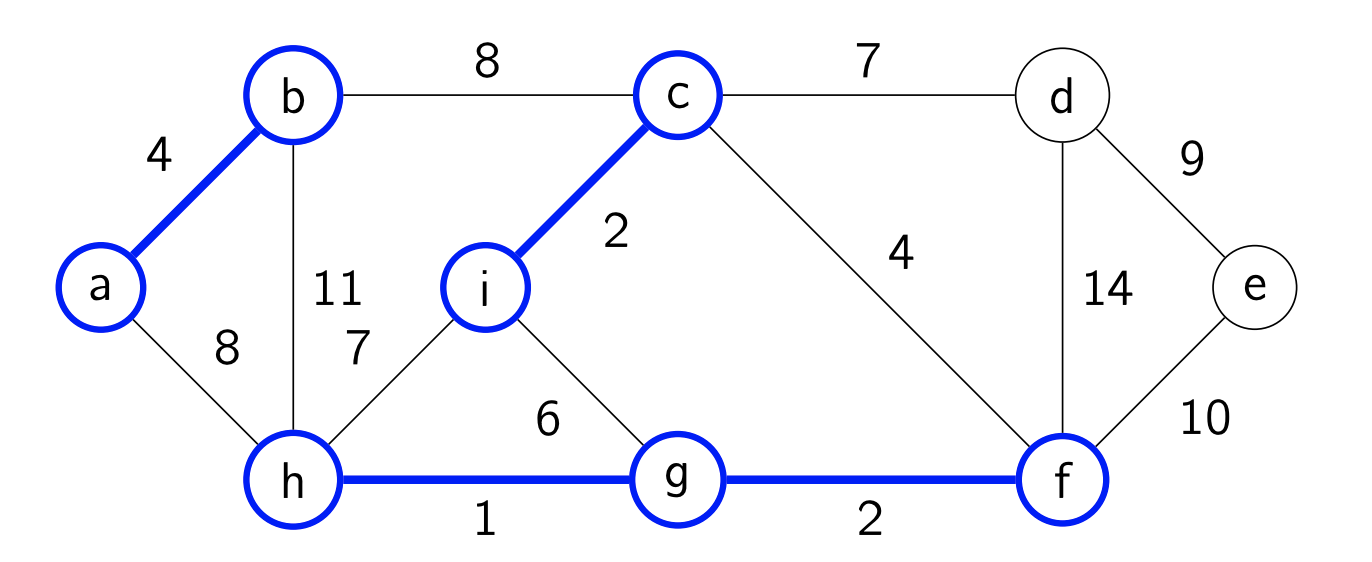
\includegraphics[scale=0.8]{kruskal4.png}
\caption{}
\label{fig:kruskal4}
\end{figure}


The next edge in the sorted order is $(c, f )$. We union the sets containing $c$ and $f$ and add edge $(c, f )$ to $A$ as shown in Figure \ref{fig:kruskal5}.

\begin{figure}[h!]
\centering
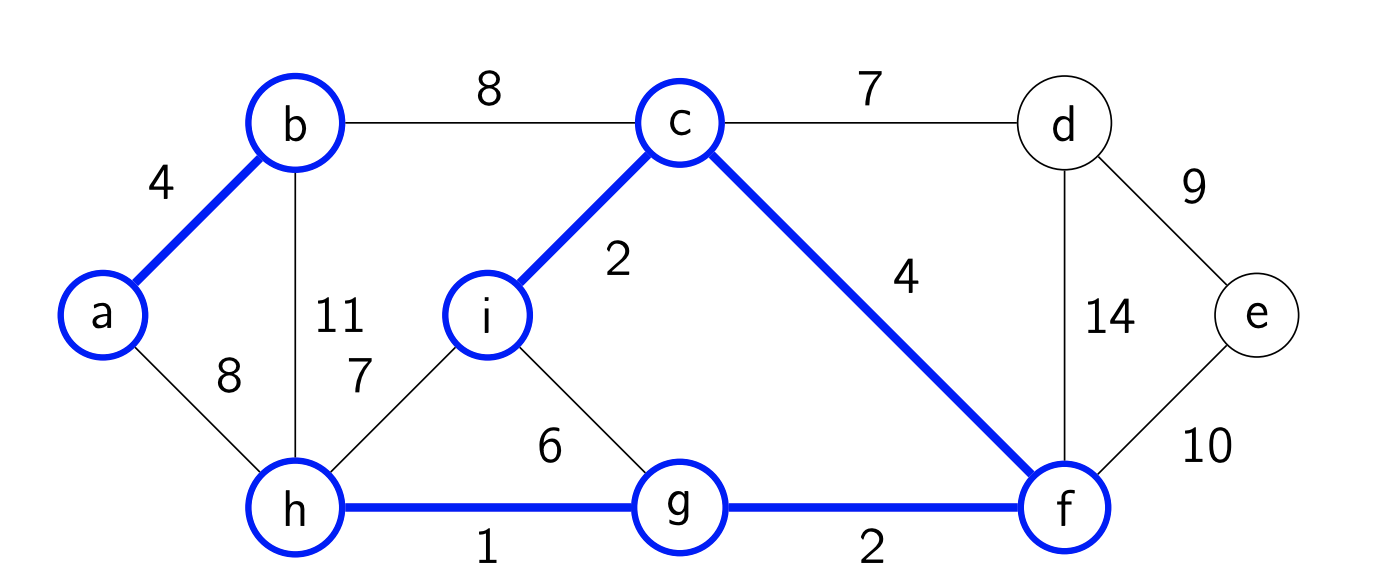
\includegraphics[scale=0.8]{kruskal5.png}
\caption{}
\label{fig:kruskal5}
\end{figure}

The next edge in the sorted order is $(i, g)$. Note that $i$ and $g$ are contained in the same set which means that adding the edge $(i, g)$ would lead to a cycle in $A$. We therefore ignore $(i, g)$ and pick the next edge in sorted order which is a tie between $(c, d)$ and $(h, i)$. Let's say the algorithm picks $(c, d)$. We union the sets containing c and d and add edge $(c, d)$ to $ A$ as shown in Figure \ref{fig:kruskal6}.

\begin{figure}[h!]
\centering
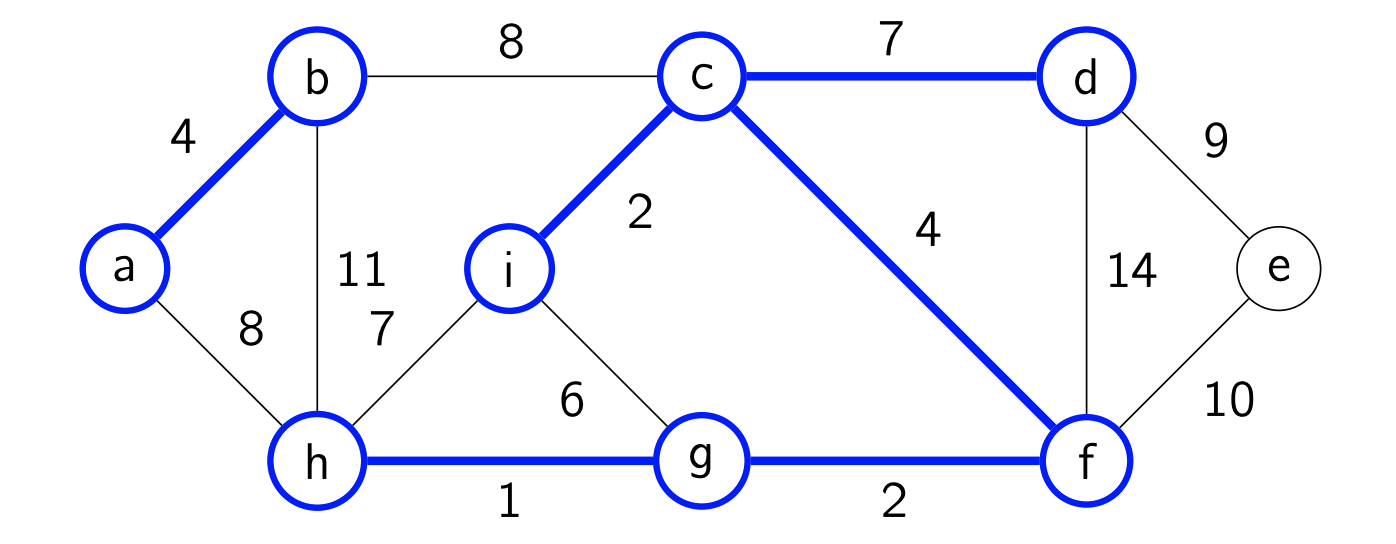
\includegraphics[scale=0.8]{kruskal6.png}
\caption{}
\label{fig:kruskal6}
\end{figure}

The next edge in the sorted order is $(h, i)$, but $h$ and $i$ are contained in the same set so we ignore it. The next edge is a tie between edges $(a, h)$ and $(b, c)$. Let's say the algorithm picks $(a, h)$. We union the sets containing a and h and add edge $(a, h)$ to $A$ as shown in Figure \ref{fig:kruskal7}.


\begin{figure}[h!]
\centering
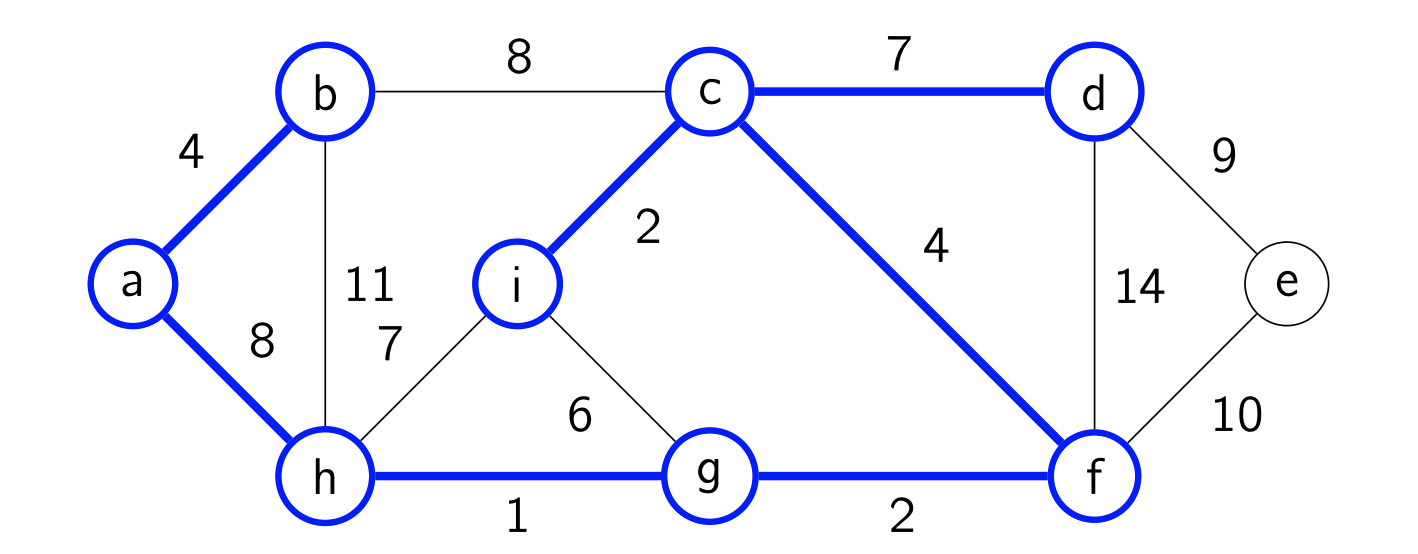
\includegraphics[scale=0.8]{kruskal7.png}
\caption{}
\label{fig:kruskal7}
\end{figure}

The next edge in the sorted order which has both vertices in different sets is $(d, e)$. We union the sets containing $ d$ and $e$ and add edge $(d, e)$ to $A$ as shown in Figure \ref{fig:kruskal8}. At this point all nodes are contained in the same set, so no further edges are added to A.


\begin{figure}[h!]
\centering
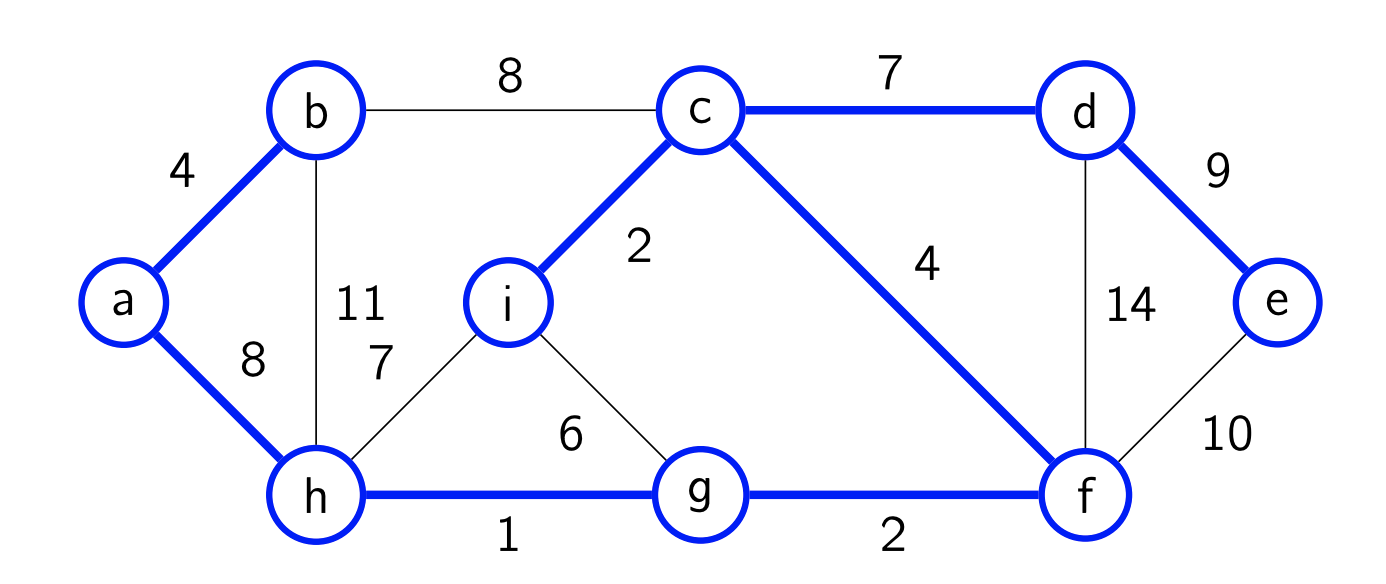
\includegraphics[scale=0.8]{kruskal8.png}
\caption{}
\label{fig:kruskal8}
\end{figure}


\section{The Latest and Greatest Algorithms}
 
While the greedy algorithms mentioned above are reasonably efficient ways to compute a minimum spanning tree of a graph, recent research has yielded more efficient algorithms. In 1995, Karger, Klein, and Tarjan discovered a randomized linear time $(O(E + V ))$ algorithm based on Borůvka's algorithm and the reverse-delete algorithm. In 2000, Chazelle discovered the current fastest determistic algorithm which runs in time $O(E \alpha(V ))$ using soft heaps where $\alpha$ is the inverse Ackermann function.


\section{History of Flows and Cuts}

Today we will study a very interesting problem called the max flow problem. Before we get to the algorithm and math, we briefly discuss the interesting history behind max flow! During the Cold War, the US Air Force at that time was very interested in the Soviet train networks. In reports that were declassified in 1999, it was revealed that the Air Force collected enough information about the train network that they were able to determine how resources were shipped from the Soviet Union to Europe. The Air Force was very interested in determining how much resources can be transported from the Soviet Union to Europe, and what needed to be done to destroy this movement of resources. What this translates to is the min cut problem, i.e., cutting the minimum number of train tracks so that nothing goes to Europe. Here, cutting an edge meant dropping a bomb. Nowadays, however, there are much more peaceful applications of this problem, for instance, understanding the flow of information through the Internet.


\section{Formulation of the Maximum Flow Problem}

You are given an input graph $G = (V, E)$, where the edges are directed. There is a function $c : E \to R\geq 0$ that defines the capacity of each edge. We also label two nodes in $G$, $s$ and $t$, as the source and destination, respectively. The task is to output a flow of maximum value. We will shortly define what a flow is and what a flow of maximum value means. 

A flow $f$ is a function $f : E \to R\geq 0$ such that 
\begin{enumerate}
    \item Capacity constraints are satisfied: 
    $$
        \forall (u, v ) \in E : 0 \leq f (u, v ) \leq c(u, v )
    $$. 
    \item Flow conservation constraints are satisfied: 
    $$
    \forall v \in V \setminus \{s, t\} : \sum_{x \in N_{\text{in}}(v)} f (x, v ) = \sum_{y\ in N_{\text{out}}(v)} f (v, y )
    $$
    Here $N_{\text{in}}(v )$ denotes the set of nodes with an edge that points to $v$ and $N_{\text{out}}(v )$ denotes the set of nodes that $v$ points to.
\end{enumerate}

\begin{figure}[h!]
    \centering
    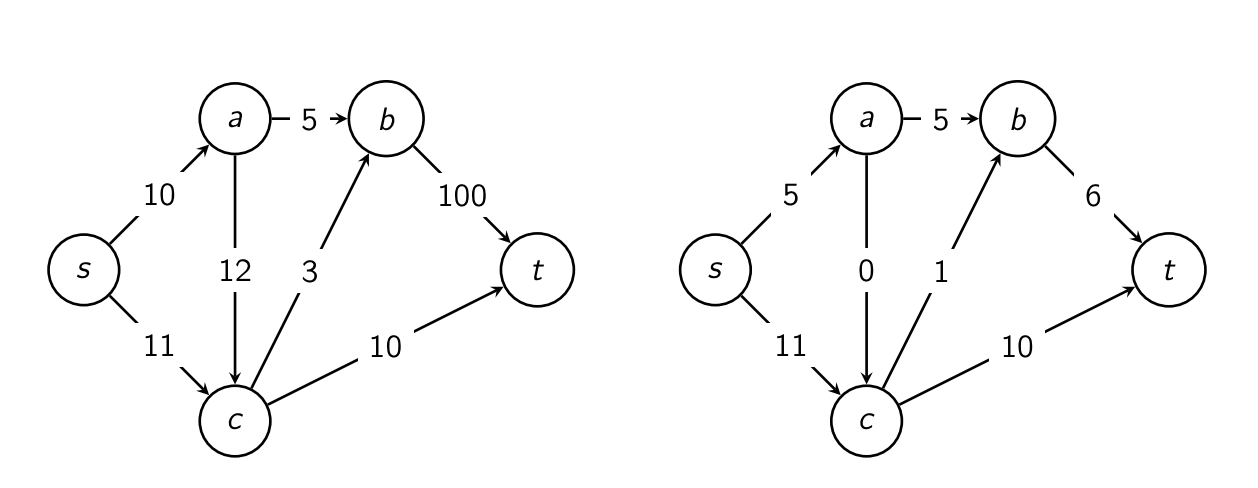
\includegraphics[scale=0.6]{max_flow_ex.png}
    \caption{(Left) Graph $G$ with edge capacities (Right) Graph $G$ with a sample flow.}
    \label{fig:max_flow_ex}
\end{figure}
 

Suppose that there are no edges going into $s$ and no edges coming out of $t$. From the above, you can verify yourself that $\sum_{x \in N_{\text{out}}(s)} f (s, x) = \sum_{y \in N_{\text{in}}(t)} f (y, t)$. We define the value $x \in N_{\text{out}}(s) f (s, x)$ to be the value of the flow $f$ . We usually denote the value of a flow $f$ as $|f |$. If there are edges going into $s$ and out of $t$, then the value of $f$ is $$
|f | = \sum_{x \in N_{\text{out}}(s)} f (s, x) - \sum_{ y \in N_{\text{in}}(s)} f (y, s)
$$.

The max flow problem is to find some flow f such that $|f |$ is maximized. Remark 1. In the analysis below we consider graphs with a single source s and a single sink t. However, if we need to work with a graph with multiple sources, we can do so by adding a new source node, and then adding edges with capacity infinity from it to each of the multiple sources. Similarly, if we want to have multiple sinks, we add a new sink node and add edges from the multiple sinks to that sink with capacity infinity.

\section{Example}

In Fig. \ref{fig:max_flow_ex}, we have a graph $G$ and a sample flow $f$ . Observe that the two constraints for a flow are satisfied. There can be multiple other flows possible that can satisfy the constraints. For our given flow, $|f | = 16$. The max flow for this graph is actually $18$, as we will see shortly.


\section{Formulation of the Minimum Cut Problem}

Now, we give a formulation of the min cut problem defined for directed graphs with source and destination nodes $s$ and $t$. Note that there is also a version of the min cut problem without a source and sink node, though we won't discuss that now. An s-t cut is a partition $V = S \cup T$ where $S$ and $T$ are disjoint and $s \in S, t \in T$, and the size/cost of an s-t cut is $c(S, T) := \sum_{x\in S, y\in T} c(x, y )$.

For our graph $G$ shown above, if we set$ S = \{s, a, c\}$ and $T = \{b, t\}$, then the cost of the cut is $c(a, b) + c(c, b) + c(c, t) = 5 + 3 + 10 = 18$. If we take another cut $S
' = \{s, c\}, T' = \{a, b, t\}$, then $c(S', T') = c(s, a) + c(c, b) + c(c, t) = 10 + 3 + 10 = 23$. Note that we do
not consider the edge $\{a, c\}$ as it is in the wrong direction (we only consider edges from $S'$ to $ T'$).


\section{The Max-Flow Min-Cut Theorem}

\begin{lemma}
For any flow $f$ and any s-t cut $(S, T)$ of $G$, we have $|f | \leq c(S, T)$. In particular,the value of the max flow is at most the value of the min cut.
\end{lemma}

\begin{proof}

\begin{align*}
|f| &= \sum_{x \in N_{\text{out}}(s)} f(s,x) - \sum_{y \in N_{\text{in}}(s)} f(y,s) \\
&=\sum_{v \in S} \left(\sum_{x \in N_{\text{out}}(v)} f(v,x) - \sum_{y \in N_{in}(v)} f(y,v) \right) \tag{by flow conservation constraing for $v \neq s$} \\
&=\sum_{v \in S} \left(\sum_{x \in N_{\text{out}}(v) \cap S} f(v,x) - \sum_{y \in N_{in}(v) \cap S} f(y,v) \right) + \sum_{v \in S} \left(\sum_{x \in N_{\text{out} \cap T}(v)} f(v,x) - \sum_{y \in N_{in}(v) \cap T} f(y,v) \right) \\
&=\sum_{v \in S} \left(\sum_{x \in N_{\text{out} \cap T}(v)} f(v,x) - \sum_{y \in N_{in}(v) \cap T} f(y,v) \right) \tag{first term sums to $0$} \\
&\leq \sum_{v \in S, x \in T, x \in N_{\text{out}}(v)} f(v,x) \\
&=\leq \sum_{v \in S, x \in T, x \in N_{\text{out}}(v)} c(v,x) \\
&= c(S,T)
\end{align*}

In the proof, $\sum_{v \in S} \left(\sum_{x\in N_{\text{out}}(v)} f(v,x) - \sum_{y\in N_{\text{int}}(v)} f(y,v)\right) = 0$ since we add and subtract the flow $f (u, v )$ for every $u, v \in S$ such that $(u, v ) \in E$.
\end{proof}

We get the following consequence.

\begin{corollary}
If we can find $f$ and $(S,T)$ such that $|f| = c(S,T)$ then $f$ is a max-flow and $(S,T)$ is a min s-t cut.
\end{corollary}

It turns out we can always find such an $f$ and $(S,T)$ for any graph.

\begin{theorem}{Max-Flow Min-cut Theorem}
For any graph $G$, source $s$ and destination $t$, the value of the max flow is equal to the cost of the min cut
\end{theorem}

We will show this by coming up with an algorithm. The algorithm will take the graph $G$ and some flow $f$ that has already been constructed, and create a new graph that is called the residual graph. In this new graph, the algorithm will try to find a path from s to t. If no such path exists, we will show that the value of the flow we started with is the value of the maximum flow. If not, we show how to increase the value of our flow by pushing some flow
on that path.

\begin{figure}[h!]
\centering
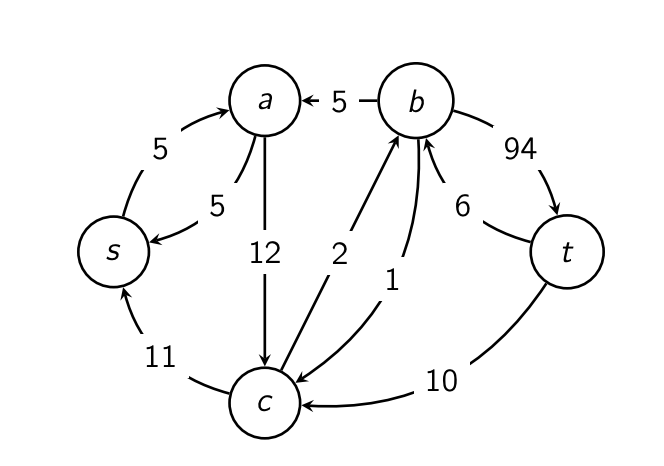
\includegraphics[scale=0.6]{max_flow_res.png}
\caption{The Residue network given the flow presented in Figure \ref{fig:max_flow_ex}}
\label{fig:max_flow_res}
\end{figure}



























\end{document}